%!TEX root = ./main.tex
%!TEX program = xelatex
% =====================================================================
%  01 - GIỚI THIỆU
% =====================================================================
\chapter{Giới thiệu}
\label{ch:gioithieu}

\section{Điều khiển động cơ DC trong đời sống và công nghiệp}

\subsection{Động cơ DC và nhu cầu điều khiển tốc độ}
Động cơ DC có chổi than (brushed DC motor) có cấu tạo đơn giản, giá thành thấp, mô-men khởi động lớn và đặc biệt là dễ điều khiển: tốc độ gần như tỉ lệ thuận với điện áp phần ứng, còn chiều quay đổi khi đảo cực tính điện áp. Nhờ đó, chỉ cần một mạch cầu H (H-bridge) và tín hiệu điều khiển thích hợp (ví dụ: PWM) là có thể điều khiển cả tốc độ lẫn chiều quay.

Tuy nhiên, khi chạy vòng hở (open-loop) -- tức chỉ đặt một mức PWM cố định -- tốc độ thực tế sẽ thay đổi khi:
\begin{itemize}
  \item tải cơ khí thay đổi (băng tải thêm hàng, robot leo dốc\ldots);
  \item điện áp nguồn dao động (pin yếu dần, nguồn công nghiệp sụt áp);
  \item nhiệt độ cuộn dây tăng làm điện trở phần ứng thay đổi;
  \item sai khác giữa các động cơ cùng loại do dung sai chế tạo.
\end{itemize}
Để giữ tốc độ ổn định, hệ thống cần một cảm biến đo tốc độ (encoder, tachometer, cảm biến Hall) và một bộ điều khiển phản hồi -- phổ biến nhất là bộ điều khiển PID. Đây là cấu trúc điều khiển vòng kín (closed-loop control).

\subsection{Ứng dụng trong đời sống}
\begin{itemize}
  \item \textbf{Thiết bị gia dụng:} máy xay sinh tố nhiều cấp tốc độ, máy hút bụi, quạt điều tốc, máy pha cà phê, bàn chải đánh răng điện.
  \item \textbf{Ô tô và xe điện cá nhân:} bơm nhiên liệu, quạt làm mát, gạt mưa, chỉnh ghế, cửa kính điện, xe đạp/xe scooter điện.
  \item \textbf{Thiết bị văn phòng và tiêu dùng:} máy in, máy quét, ổ đĩa, đồ chơi điều khiển từ xa, drone cỡ nhỏ.
  \item \textbf{Y tế:} bơm tiêm điện, bơm truyền dịch, máy thở -- nơi lưu lượng phải chính xác nên bắt buộc điều khiển vòng kín.
  \item \textbf{Giáo dục và nghiên cứu:} robot dò line, robot tự cân bằng, mô hình thí nghiệm điều khiển tự động.
\end{itemize}

\subsection{Ứng dụng trong công nghiệp}
\begin{itemize}
  \item \textbf{Băng tải và hệ thống phân loại:} giữ tốc độ băng tải không đổi khi tải thay đổi để đồng bộ với camera, cảm biến và cơ cấu gắp.
  \item \textbf{Robot di động (AGV/AMR):} điều khiển tốc độ từng bánh xe để xe đi đúng quỹ đạo; tính toán quãng đường từ encoder (odometry).
  \item \textbf{Máy CNC, máy in 3D, cánh tay robot:} servo DC có encoder điều khiển vị trí và tốc độ chính xác.
  \item \textbf{Bơm, quạt, máy khuấy công nghiệp:} điều khiển lưu lượng/áp suất thông qua tốc độ động cơ, tiết kiệm năng lượng.
  \item \textbf{Dây chuyền cuốn -- nhả (winding):} điều khiển tốc độ và lực căng cho giấy, màng nhựa, dây cáp.
\end{itemize}
Trong công nghiệp, các chức năng trên thường được đảm nhiệm bởi bộ điều khiển động cơ (motor driver/controller) chuyên dụng, nhận lệnh từ PLC hoặc máy tính qua tín hiệu tương tự (0--10 V, chiết áp), xung PWM hoặc các bus truyền thông (UART/RS-485, CAN, Modbus). Một bộ điều khiển như vậy luôn có các khối: nguồn và bảo vệ, tầng công suất, đo phản hồi, bộ xử lý chạy thuật toán điều khiển, giao diện người dùng và giao tiếp. \proj{} được thiết kế đúng theo cấu trúc đó, ở quy mô thu nhỏ phù hợp với một đề tài học phần.

\section{Tổng quan về \proj}

\subsection{\proj{} là gì?}
\textbf{\proj} là một \textbf{bộ điều khiển tốc độ động cơ DC có chổi than, vòng kín, một kênh}, được xây dựng trên vi điều khiển AVR 8-bit \textbf{ATmega88PA} chạy ở \SI{16}{\mega\hertz}. Toàn bộ hệ thống nằm trên một bo mạch in 2 lớp kích thước 80\,$\times$\,60\,mm, sử dụng một nguồn duy nhất \SI{12}{\volt} DC.

Tên gọi ``UniDrive'' (\emph{Universal Drive}) thể hiện định hướng của nhóm: một bộ điều khiển \emph{đa dụng}, có thể dùng cho nhiều loại động cơ DC có encoder khác nhau chỉ bằng cách thay đổi các thông số trong một tệp cấu hình duy nhất (\texttt{config.h}). Hậu tố ``Lite'' cho biết đây là phiên bản rút gọn, đặt nền móng cho phiên bản đầy đủ \projpro{} (xem Chương~\ref{ch:ketluan}).

\subsection{\proj{} làm được gì?}
\begin{itemize}
  \item \textbf{Điều khiển tốc độ vòng kín} bằng bộ PID số dấu phẩy tĩnh (Q8) có bù thuận (feed-forward), giới hạn gia tốc (setpoint ramp), chống bão hòa tích phân (anti-windup) và lọc thành phần vi phân.
  \item \textbf{Điều khiển hai chiều quay}, dải đặt tốc độ $\pm\SI{2700}{rpm}$ (cấu hình được).
  \item \textbf{Đo tốc độ} bằng encoder cầu phương, giải mã $\times4$, có bộ lọc số chống nhiễu kiểu ``STM32 input filter''.
  \item \textbf{Hai chế độ đặt tốc độ:}
    \begin{itemize}
      \item \emph{POTENTIOMETER} -- xoay chiết áp: vị trí giữa là \SI{0}{rpm}, xoay về hai phía để đổi chiều quay;
      \item \emph{UART} -- gửi lệnh số nguyên từ máy tính/PLC/vi điều khiển khác ở \SI{115200}{baud}.
    \end{itemize}
  \item \textbf{Giao diện người dùng:} 2 nút nhấn RUN/STOP (nhấn ngắn/nhấn giữ), 2 LED trạng thái và màn hình TFT màu 1,8\,inch hiển thị chế độ, trạng thái, tốc độ đặt và tốc độ đo được.
  \item \textbf{Bảo vệ:} chống ngược cực nguồn bằng P-MOSFET, các bảo vệ quá dòng/quá nhiệt/thấp áp tích hợp trong IC công suất, chế độ ngủ (sleep) ngắt hoàn toàn tầng công suất khi dừng.
\end{itemize}

\section{Sơ đồ khối phần cứng}

Hình~\ref{fig:sodokhoi} trình bày sơ đồ khối phần cứng của \proj. Hệ thống gồm năm nhóm chức năng: \textcolor{hustred}{\textbf{nguồn}}, \textcolor{blk}{\textbf{xử lý trung tâm}}, \textbf{tầng công suất}, \textcolor{green!40!black}{\textbf{giao diện vào/ra}} và \textbf{giao tiếp/nạp chương trình}.

\begin{figure}[H]
\centering
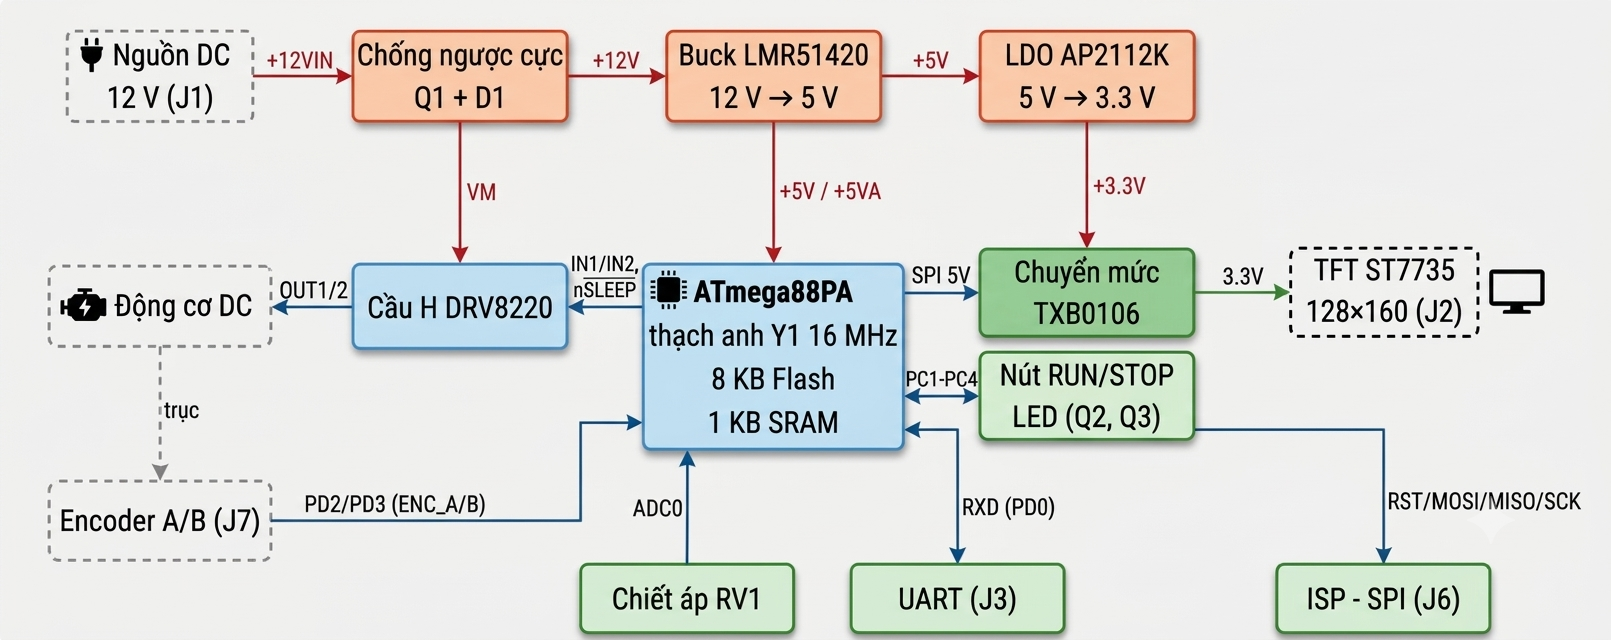
\includegraphics[width=\linewidth]{figures/SODOKHOIHARDWARE.png}
\caption{Sơ đồ khối phần cứng của \proj}
\label{fig:sodokhoi}
\end{figure}

\begin{figure}[H]
\centering
\begin{subfigure}{0.49\linewidth}\centering\hinh[\linewidth]{figures/3D_Front.png}{Ảnh 3D mặt trên}\caption{Mặt trên}\end{subfigure}
\hfill
\begin{subfigure}{0.49\linewidth}\centering\hinh[\linewidth]{figures/3D_Back.png}{Ảnh 3D mặt dưới}\caption{Mặt dưới}\end{subfigure}
\caption{Mô hình 3D bo mạch \proj{} (xuất từ KiCad)}
\label{fig:3d}
\end{figure}

\section{Danh sách linh kiện}

Bảng~\ref{tab:bom} liệt kê các linh kiện chính, được nhóm theo khối chức năng. Danh sách đầy đủ (bao gồm tụ, trở thụ động) được trích trực tiếp từ sơ đồ nguyên lý KiCad.

\begin{longtable}{@{}p{2.6cm}p{3.4cm}p{3.4cm}c p{3.4cm}@{}}
\caption{Danh sách linh kiện (BOM) của \proj}\label{tab:bom}\\
\toprule
\textbf{Ký hiệu} & \textbf{Giá trị / Mã} & \textbf{Vỏ (footprint)} & \textbf{SL} & \textbf{Chức năng}\\
\midrule\endfirsthead
\toprule
\textbf{Ký hiệu} & \textbf{Giá trị / Mã} & \textbf{Vỏ (footprint)} & \textbf{SL} & \textbf{Chức năng}\\
\midrule\endhead
\bottomrule\endfoot
\multicolumn{5}{@{}l}{\cellcolor{blkfill}\textit{Khối xử lý trung tâm}}\\
U2 & ATmega88PA-A & TQFP-32 & 1 & Vi điều khiển chính\\
Y1 & \SI{16}{\mega\hertz} & SMD 3225 & 1 & Thạch anh dao động\\
C7, C8 & \SI{22}{\pico\farad} & 0603 & 2 & Tụ tải thạch anh\\
L1 / R1 & \SI{10}{\micro\henry} / \SI{22}{\ohm} & 0603 & 2 & Lọc nguồn AVCC (+5VA)\\
C1--C3, C6 & \SI{100}{\nano\farad}, \SI{10}{\nano\farad} & 0603 & 4 & Tụ thoát VCC/AVCC/AREF\\
SW3, R6, C21 & Nút nhấn, \SI{10}{\kilo\ohm}, \SI{100}{\nano\farad} & B3F, 0603 & 3 & Mạch RESET\\
\multicolumn{5}{@{}l}{\cellcolor{pwrfill}\textit{Khối nguồn và bảo vệ}}\\
Q1 & CSD25404Q3 & VSON-8 3,3$\times$3,3 & 1 & P-MOSFET chống ngược cực\\
D1 & BZT52C10 & SOD-123 & 1 & Zener kẹp $V_{GS}$ của Q1\\
R2 & \SI{100}{\kilo\ohm} & 0603 & 1 & Điện trở cực cổng Q1\\
U1 & LMR51420XFDDCR & SOT-23-6 & 1 & Buck đồng bộ \SI{12}{\volt}$\to$\SI{5}{\volt}\\
L2 & \SI{10}{\micro\henry} & IHLP-1616 & 1 & Cuộn cảm buck\\
R5, R7 & \SI{100}{\kilo\ohm}, \SI{13.7}{\kilo\ohm} & 0603 & 2 & Cầu phân áp hồi tiếp (FB)\\
C9, C10, C11, C12 & \SI{100}{\nano\farad}, \SI{2.2}{\micro\farad}, 2$\times$\SI{22}{\micro\farad} & 0603/1206 & 4 & Bootstrap, tụ vào, tụ ra\\
U3 & AP2112K-3.3 & SOT-23-5 & 1 & LDO \SI{3.3}{\volt} / \SI{600}{\milli\ampere}\\
C13, C14 & \SI{22}{\micro\farad} & 1206 & 2 & Tụ vào/ra LDO\\
C4, C17 & \SI{220}{\micro\farad} & Hóa 6,3$\times$7,7 & 2 & Tụ bulk bus \SI{12}{\volt}\\
\multicolumn{5}{@{}l}{\cellcolor{blkfill}\textit{Khối công suất}}\\
U5 & DRV8220DSG & WSON-8 2$\times$2 & 1 & Cầu H \SI{18}{\volt}/\SI{1.76}{\ampere}\\
JP1, R10 & Jumper hàn, \SI{10}{\kilo\ohm} & -- & 2 & Chọn chế độ PWM / PH-EN\\
C18 & \SI{100}{\nano\farad} & 0603 & 1 & Tụ thoát VM\\
M1 & Domino 2 chân & MKDS 5,08 & 1 & Đầu ra động cơ\\
\multicolumn{5}{@{}l}{\cellcolor{iofill}\textit{Khối giao diện}}\\
U4 & TXB0106RGY & VQFN-16 & 1 & Chuyển mức \SI{5}{\volt}$\leftrightarrow$\SI{3.3}{\volt} cho TFT\\
R9, R12 & \SI{30.1}{\kilo\ohm}, \SI{60.4}{\kilo\ohm} & 0603 & 2 & Phân áp chân OE\\
C15, C16 & \SI{100}{\nano\farad} & 0603 & 2 & Tụ thoát VCCA/VCCB\\
RV1 & Chiết áp Alps RK097 & -- & 1 & Đặt tốc độ\\
SW1, SW2 & Nút nhấn Omron B3F & -- & 2 & Nút RUN, STOP\\
R3, R4, C19, C20 & \SI{10}{\kilo\ohm}, \SI{100}{\nano\farad} & 0603 & 4 & Kéo xuống + lọc RC nút nhấn\\
D2, D3 & LED & 1206 & 2 & LED STOP, RUN\\
Q2, Q3 & 2N7002 & SOT-23 & 2 & Khóa LED\\
R8, R11, R13--R16 & \SI{10}{\kilo\ohm}, \SI{22}{\ohm} & 0603 & 6 & Trở hạn dòng LED, trở cổng\\
\multicolumn{5}{@{}l}{\cellcolor{swfill}\textit{Đầu nối và cơ khí}}\\
J1 & Domino 2 chân & MKDS 5,08 & 1 & Đầu vào nguồn \SI{12}{\volt}\\
J2 & Header cái 1$\times$8 & 2,54 mm & 1 & Module TFT WeAct ST7735\\
J3 & JST-XH 4 chân & 2,50 mm & 1 & UART\\
J6 & JST-XH 5 chân & 2,50 mm & 1 & Nạp ISP\\
J7 & JST-XH 4 chân & 2,50 mm & 1 & Encoder\\
J4, J5 & Header 1$\times$3 & 2,54 mm & 2 & Đầu chờ +5V / GND\\
TP1--TP7 & Test point & $\varnothing$\SI{1}{\milli\metre} & 7 & Điểm đo\\
H1--H4 & Lỗ M3 & $\varnothing$\SI{3.2}{\milli\metre} & 4 & Lỗ bắt vít\\
\end{longtable}

\section{Thông số kỹ thuật}
\label{sec:thongso}

Phần này trình bày thông số của \proj{}. Các giới hạn được suy ra từ datasheet của linh kiện yếu nhất trong mỗi đường tín hiệu; các thông số chức năng được tính từ cấu hình firmware mặc định trong \texttt{config.h}.

\begin{tcolorbox}[colback=white,colframe=hustred,title={\bfseries UNIDRIVE LITE -- Single-Channel Closed-Loop Brushed DC Motor Controller},fonttitle=\large]
\begin{minipage}[t]{0.48\linewidth}
\textbf{Đặc điểm nổi bật}
\begin{itemize}[leftmargin=*,itemsep=0pt]
  \item Nguồn vào đơn \SIrange{7}{16}{\volt}, danh định \SI{12}{\volt}
  \item Chống ngược cực nguồn
  \item Dòng động cơ đỉnh \SI{1.76}{\ampere}
  \item PID dấu phẩy tĩnh, chu kỳ \SI{50}{\milli\second}
  \item Encoder $\times4$ có lọc nhiễu số
\end{itemize}
\end{minipage}\hfill
\begin{minipage}[t]{0.48\linewidth}
\textbf{\phantom{x}}
\begin{itemize}[leftmargin=*,itemsep=0pt]
  \item Đặt tốc độ: chiết áp / UART
  \item Màn hình TFT màu 128$\times$160
  \item Cấu hình tập trung trong \texttt{config.h}
  \item Bo mạch 2 lớp 80\,$\times$\,60\,mm
  \item Nạp chương trình qua ISP (SPI)
\end{itemize}
\end{minipage}
\end{tcolorbox}

\subsection{Giới hạn tuyệt đối (Absolute Maximum Ratings)}
\begin{table}[H]
\centering\small
\caption{Giới hạn tuyệt đối -- vượt quá có thể làm hỏng thiết bị}
\label{tab:absmax}
\begin{tabularx}{\linewidth}{@{}Xccc>{\raggedright\arraybackslash}p{4.2cm}@{}}
\toprule
\textbf{Thông số} & \textbf{Min} & \textbf{Max} & \textbf{Đơn vị} & \textbf{Giới hạn bởi}\\
\midrule
Điện áp vào $V_{IN}$ (J1) & $-20$ & 20 & \si{\volt} & $V_{DS}$ Q1, $V_{M}$ DRV8220\\
Dòng ra động cơ (đỉnh) & -- & 1,76 & \si{\ampere} & Giới hạn dòng DRV8220\\
Tải trên đường \SI{5}{\volt} (J4) & -- & 2 & \si{\ampere} & LMR51420 (gồm tải nội)\\
Tải trên đường \SI{3.3}{\volt} & -- & 0,6 & \si{\ampere} & AP2112K\\
Điện áp chân tín hiệu J3, J7 & $-0,5$ & 5,5 & \si{\volt} & ATmega88PA ($V_{CC}+0,5$)\\
Điện áp chân MODE (DRV8220) & -- & 5,75 & \si{\volt} & DRV8220\\
Nhiệt độ làm việc & $-20$ & 85 & \si{\celsius} & Linh kiện thương mại\\
\bottomrule
\end{tabularx}
\end{table}

\subsection{Điều kiện làm việc khuyến nghị}
\begin{table}[H]
\centering\small
\caption{Điều kiện làm việc khuyến nghị}
\label{tab:recommended}
\begin{tabularx}{\linewidth}{@{}Xcccc@{}}
\toprule
\textbf{Thông số} & \textbf{Min} & \textbf{Typ} & \textbf{Max} & \textbf{Đơn vị}\\
\midrule
Điện áp vào $V_{IN}$ (in trên bo: MAX 16\,VDC) & 7 & 12 & 16 & \si{\volt}\\
Dòng động cơ liên tục & -- & -- & 1,0 & \si{\ampere}\\
Điện áp định mức động cơ & -- & $V_{IN}$ & -- & \si{\volt}\\
Độ phân giải encoder  & 1 & 20 & 500 & PPR\\
Tần số mỗi kênh encoder (khi bật lọc) & 0 & -- & 5 & \si{\kilo\hertz}\\
\bottomrule
\end{tabularx}
\end{table}

\subsection{Đặc tính điện}
\begin{table}[H]
\centering\small
\caption{Đặc tính điện ($V_{IN}=\SI{12}{\volt}$, $T_A=\SI{25}{\celsius}$, cấu hình mặc định)}
\label{tab:electrical}
\begin{tabularx}{\linewidth}{@{}>{\raggedright\arraybackslash}Xp{3.6cm}cccc@{}}
\toprule
\textbf{Thông số} & \textbf{Điều kiện} & \textbf{Min} & \textbf{Typ} & \textbf{Max} & \textbf{Đơn vị}\\
\midrule
\multicolumn{6}{@{}l}{\textit{Nguồn}}\\
Điện áp đường +5V & $I_{OUT}\le\SI{1}{\ampere}$ & 4,92 & 4,98 & 5,05 & \si{\volt}\\
Điện áp đường +3.3V & -- & 3,23 & 3,30 & 3,37 & \si{\volt}\\
Tần số chuyển mạch buck & FPWM & -- & 500 & -- & \si{\kilo\hertz}\\
Sụt áp chống ngược cực & $I=\SI{1}{\ampere}$ & -- & 5,5 & -- & \si{\milli\volt}\\
Dòng tiêu thụ khi STOP & Động cơ ngủ & -- & \bosung{đo} & -- & \si{\milli\ampere}\\
\multicolumn{6}{@{}l}{\textit{Tầng công suất}}\\
Tần số PWM & Timer2, chia 32 & -- & 1953 & -- & \si{\hertz}\\
Độ phân giải PWM & -- & -- & 8 & -- & bit\\
Chế độ suy giảm dòng & Mặc định & \multicolumn{3}{c}{Slow decay (hãm)} & --\\
\multicolumn{6}{@{}l}{\textit{Đo lường và điều khiển}}\\
Dải đặt tốc độ & \texttt{APP\_MAX\_RPM} & $-2700$ & -- & 2700 & \si{rpm}\\
Độ phân giải đo tốc độ & 20 PPR, cửa sổ \SI{50}{\milli\second} & -- & 15 & -- & \si{rpm}\\
Chu kỳ vòng điều khiển & \texttt{MOTION\_PERIOD\_MS} & -- & 50 & -- & \si{\milli\second}\\
Giới hạn gia tốc đặt & \texttt{MOTION\_ACCEL} & -- & 6000 & -- & \si{rpm\per\second}\\
Độ rộng xung nhiễu bị loại & $N=4$, \SI{80}{\kilo\hertz} & -- & 50 & -- & \si{\micro\second}\\
\multicolumn{6}{@{}l}{\textit{Giao diện}}\\
Tốc độ UART & 8N1, chỉ nhận & -- & 115200 & -- & baud\\
Sai số tốc độ baud & U2X, UBRR = 16 & -- & +2,1 & -- & \%\\
Độ phân giải ADC chiết áp & Tham chiếu AVCC & -- & 10 & -- & bit\\
Thời gian chống dội nút & -- & -- & 20 & -- & \si{\milli\second}\\
Thời gian nhấn giữ & -- & -- & 2000 & -- & \si{\milli\second}\\
Xung nhịp SPI tới TFT & $f_{osc}/2$ & -- & 8 & -- & \si{\mega\hertz}\\
\bottomrule
\end{tabularx}
\end{table}

\subsection{Sơ đồ chân đầu nối}
\begin{table}[H]
\centering\small
\caption{Sơ đồ chân các đầu nối trên bo mạch}
\label{tab:connectors}
\begin{tabularx}{\linewidth}{@{}l>{\raggedright\arraybackslash}p{2.8cm}c>{\raggedright\arraybackslash}X@{}}
\toprule
\textbf{Đầu nối} & \textbf{Chức năng} & \textbf{Chân} & \textbf{Tín hiệu}\\
\midrule
J1 & Nguồn vào & 1 / 2 & +12VIN / GND\\
M1 & Động cơ & 1 / 2 & OUT1 (+) / OUT2 ($-$)\\
J2 & TFT ST7735 & 1--8 & GND, +5V, SCK, SDA, RST, DC, CS, BL (mức \SI{3.3}{\volt})\\
J3 & UART & 1--4 & +5V, RX (PD0), GND, TX (PD1)\\
J6 & ISP & 1--5 & RESET, MOSI, MISO, SCK, GND \textit{(không cấp nguồn)}\\
J7 & Encoder & 1--4 & +5V, ENC\_A (PD2), ENC\_B (PD3), GND\\
J4 / J5 & Đầu chờ & 1--3 & +5V / GND\\
\bottomrule
\end{tabularx}
\end{table}

\subsection{Phân bố chân vi điều khiển}
\begin{table}[H]
\centering\small
\caption{Phân bố chân ATmega88PA}
\label{tab:pinmap}
\begin{tabular}{@{}lll|lll@{}}
\toprule
\textbf{Chân} & \textbf{Tín hiệu} & \textbf{Ngoại vi} & \textbf{Chân} & \textbf{Tín hiệu} & \textbf{Ngoại vi}\\
\midrule
PB0 & TFT\_RST & GPIO & PD0 & UART RX & USART0\\
PB1 & TFT\_BL & GPIO & PD2 & ENC\_A & Timer1 lấy mẫu\\
PB2 & TFT\_CS & GPIO & PD3 & ENC\_B & Timer1 lấy mẫu\\
PB3 & TFT\_MOSI & SPI & PD4 & nSLEEP & GPIO\\
PB5 & TFT\_SCK & SPI & PD5 & IN1/PH & PWM mềm Timer2\\
PB6/PB7 & XTAL1/2 & Thạch anh & PD6 & IN2/EN & PWM mềm Timer2\\
PC0 & Chiết áp & ADC0 & PD7 & TFT\_DC & GPIO\\
PC1 / PC3 & Nút RUN / STOP & GPIO & PC6 & RESET & ISP\\
PC2 / PC4 & LED RUN / STOP & GPIO & ADC6 & OE\_CONTROL & (xem mục~\ref{sec:hanche})\\
\bottomrule
\end{tabular}
\end{table}
